%\documentclass[english,twoside]{article}
\documentclass[english,twoside]{labmanual} 
%labmanual.cls is a modified version of article.cls, tweaked to handle \part{} differently

%% LyX 1.1 created some parts of this file.  For more info, see http://www.lyx.org/.
%% Do not edit unless you really know what you are doing.

\usepackage[T1]{fontenc}
\usepackage[nomarginpar]{geometry}
\usepackage{tocloft} %Allow us to leave page numbers for Parts out of table of contents
\cftpagenumbersoff{part} %No page numbers for Parts out of table of contents
\renewcommand{\cftsecdotsep}{\cftsubsecdotsep}
%\usepackage{newclude} %Allows use of /include*{}
%DANGER DANGER: newclude is NOT compatible with package xr, used for external references.
\geometry{verbose,letterpaper}
\usepackage{fancyhdr}
\usepackage{babel}
\setlength\parskip{\medskipamount}
\setlength\parindent{0pt}
\usepackage{graphicx}
\usepackage{wrapfig}
%\usepackage{epstopdf} %this package apparently allows pdflatex to work on this document, since all we use are eps figures.
\usepackage{comment}
\usepackage{esvect}
\usepackage{amsmath} %uncommented by MT 5/2015, used in "E near charged rod"
\usepackage{mathtools} %added by MT 6/2015, for access to dcases environment in finding_v_from_e
\usepackage{tabularx} %added by MT 6/2015, for fixed width columns, used in rc_circuits
\usepackage{microtype}
\usepackage{titlesec}
\usepackage{xr}

%For fixed width columns:
\newcolumntype{L}[1]{>{\raggedright\arraybackslash}p{#1}}
\newcolumntype{C}[1]{>{\centering\arraybackslash}p{#1}}
\newcolumntype{R}[1]{>{\raggedleft\arraybackslash}p{#1}}


\addtolength{\oddsidemargin}{1.0cm} %without these two lines, larger margin is on the OUTSIDE.  We want the larger edge on the INSIDE, to allow room for the three hole punches
\addtolength{\evensidemargin}{-1.0cm}

\setlength\topmargin{0.2in}
\addtolength{\hoffset}{-1.0cm}
\addtolength{\textwidth}{2.0cm}
\addtolength{\voffset}{-1.5cm} %This line is apparently needed on some versions of MikTex XeLatex.  Comment out if your pages appear shifted too high.
\addtolength{\textheight}{3.5cm}
% define a strut for extra vertical space in tables.
\newcommand{\hi}{\rule[-2mm]{0mm}{6mm}}

\pagestyle{fancy}
%\fancyhead[LE,RO]{\slshape \rightmark} %This is the default for fancy page style
%\fancyhead[LO,RE]{\slshape \leftmark}
\fancyhead[LO,RE]{\slshape \rightmark} 
\fancyhead[LE,RO]{\slshape \leftmark} % Reversed LE, RO to  LO,RE to make headers come out correctly on even/odd pages



%%%%%%%%%%%%%%%%%%%%%%%%%%%%%% LyX specific LaTeX commands.
\providecommand{\LyX}{L\kern-.1667em\lower.25em\hbox{Y}\kern-.125emX\@}
\newenvironment{LyXParagraphIndent}[1]%
{
  \begin{list}{}{%
    \setlength\topsep{0pt}%
    \addtolength{\leftmargin}{#1}
    \setlength\parsep{0pt plus 1pt}%
  }
  \item[]
}
{\end{list}}
%% Special footnote code from the package 'stblftnt.sty'
%% Author: Robin Fairbairns -- Last revised Dec 13 1996
\makeatletter
\let\SF@@footnote\footnote
\def\footnote{\ifx\protect\@typeset@protect
    \expandafter\SF@@footnote
  \else
    \expandafter\SF@gobble@opt
  \fi
}
\expandafter\def\csname SF@gobble@opt \endcsname{\@ifnextchar[%]
  \SF@gobble@twobracket
  \@gobble
}
\edef\SF@gobble@opt{\noexpand\protect
  \expandafter\noexpand\csname SF@gobble@opt \endcsname}
\def\SF@gobble@twobracket[#1]#2{}
\makeatother


%I make use of some latex features to manage the section numbers. To use those you have to insert the following lines into the latex preamble (before the %"\begin{document}" command).

% two new commands to do labelling. - gpg 12/4/13
\newcommand{\customlabel}[2]{%
\protected@write \@auxout {}{\string \newlabel {#1}{{#2}{}}}}

\newcommand{\actlabel}[1]{%
\protected@write \@auxout {}{\string \newlabel {#1}{{\arabic{activity}}{}}}}

\newcommand{\makelabheader}
%{Name: \rule{2.0in}{0.1pt}\hfill{}Section: \rule{1.0in}{0.1pt}\hfill{}Date: \rule{1.0in}{0.1pt}}
{Name: \rule{2.0in}{0.1pt}\hfill{}Lab Partner(s): \rule{3.0in}{0.1pt}}

%\newcommand{\dir131}{../../131/StudentGuideModule1} %This does not work, because commands can only be made of numeric characters, not numbers.

%A new command for putting a box around a paragraph:
\newenvironment{newboxed} %maybe there's a better way to do this.  I just cribbed from the web. --MT
    {\begin{center}
    \begin{tabular}{|p{0.9\textwidth}|}
    \hline\\
    }
    { 
    \\\\\hline
    \end{tabular} 
    \end{center}
    }

\newcounter{activity}

%  The following command, \answerspace, should be used to replace \vspace.
%  \vspace{} is not ideal for an answer space for students, for two reasons:
%  1. It can be ignored if it comes at the end of a page, and
%  2. The spacing is exact, and Latex will not stretch or compress it at all to make things fit on a page, which means
%  that other things WILL get stretched or compressed to make things fit, which means those other things will 
%  end up looking bad, and leading to a lot of underfull \vbox warnings.
%  \answerspace fixes both of those problems, specifically allowing the space to grow to up to twice the stated size.
\newcommand{\answerspace}[1]{\vspace*{#1 plus #1}}

%  The next several lines implement \includelab, which replaces \include.
%  Usage is \includelab{1}{file} to include it, or \includelab{0}{file} to NOT include it.  
%  But all 0's can be overridden by writing \includealllabstrue in the master.tex file, which is easier than deleting 
%  fifty individual `%' signs and then remembering to put them all back, which is what you had to do before.
%  \includeonly still works as you expect it to.
\newif\ifincludealllabs
\newcommand{\includelab}[2]{
	\ifnum#1=1
		\include{#2}
	\else {
		\ifincludealllabs
		 	\include{#2}
		\fi}
	\fi
}
 %all general latex packages, commands, and definitions now here.
\externaldocument{master}

%syntax: \includeonly{lab1,lab2,lab3} with no spaces after the commas.
%\includeonly{biot_savart_law/biot_savart_law, charge_density/charge_density,eoverm/eoverm }
%DANGER: The includeonly statement will make a document that does NOT have sequential page numbers.

\newcommand{\supplementmark}{JS}

\titleformat{\section}{\normalfont\Large\bfseries}{\supplementmark \thesection}{1em}{}
\fancyhead[LO,RE]{\slshape \rightmark} 
\fancyhead[LE,RO]{\slshape \supplementmark \leftmark} % Reversed LE, RO to  LO,RE to make headers come out correctly on even/odd 

\begin{document}

\setcounter{page}{157}  %Set this to desired first page
\setcounter{section}{37} %set this to desired first section number MINUS ONE

%--------------------------------------------
%Put include statements for labs below here.

\section{Capacitance Series Circuit}

Name \rule{2.0in}{0.1pt}\hfill{}Section \rule{1.0in}{0.1pt}\hfill{}Date
\rule{1.0in}{0.1pt}

\textbf{Objective}

\begin{itemize}
\item To investigate the relationship among charge, potential difference, and capacitance in a series combination of capacitors.
\end{itemize}
\textbf{Introduction} 

In class the series combination of capacitors was studied with the assumption
of a constant potential difference energizing the circuit.  In practice this
is difficult to reproduce in the lab because capacitors typically do not
maintain a steady charge for very long.  To get around this we will energize
the circuit with an alternating potential difference provided by a sine wave
generator.  The relationships among $Q$, $V$, and $C$ are still the same, so
we can study these circuits in the lab.

For a series combination of capacitors, the total voltage across the circuit
is the sum of the voltages across the individual capacitors, that is

\begin{displaymath} V = V_1 + V_2 + V_3 \end{displaymath}

The equivalent capacitance of the combination is given by

\begin{displaymath} \frac{1}{C} = \frac{1}{C_1} + \frac{1}{C_2} + \frac{1}{C_3} \end{displaymath}

\textbf{Apparatus}

\begin{itemize}
\item Sine wave generator 
\item Capacitors of 1.0, 4.7, and 10 $\mu$f
\item Digital multimeter
\item Connecting leads
\end{itemize}
\textbf{Activity}

%\vspace{0.3cm}
%{\centering \resizebox*{0.45\textwidth}{!}{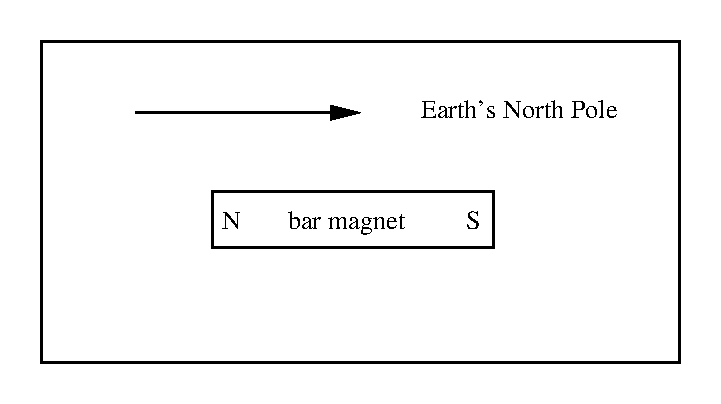
\includegraphics{magnetism_2_fig_1.eps}} \par}
%\vspace{0.3cm}

\begin{enumerate}
\item Connect the three capacitors in series with the sine wave generator.
\item Set the sine wave generator to 200 Hz (not critical) and adjust the
amplitude so that the output measures 5 to 6 volts as measured with the
digital multimeter set for \underline{AC volts}.
\item Using the multimeter, measure $V$ for the sine wave generator and also
for each of the individual capacitors (all with uncertainties) and
list them here. Don't forget units.\vspace{20mm}
\item Calculate the total voltage and its uncertainty from the first equation
above and compare with your measured value.  Do they agree?\vspace{30mm}
\item Assuming 10 percent uncertainties on each of the capacitances,
calculate the equivalent capacitance and its uncertainty from the second
equation above.\vspace{30mm}
\item Calculate the total charge for the circuit (and its uncertainty) from
$Q = CV$.\vspace{30mm}
\item \textbf{Prediction:} How will the charge on the individual capacitors
compare with the total charge calculated above?\vspace{30mm}
\item Calculate the charge on each capacitor (and its uncertainty) and compare with the total.
Do the results agree with your prediction?
\end{enumerate}


\section{Boyle's Law}

Name \rule{2.0in}{0.1pt}\hfill{}Section \rule{1.0in}{0.1pt}\hfill{}Date
\rule{1.0in}{0.1pt}

\textbf{Objective}

%test comment

To investigate the relationship between the pressure and volume of
a gas.

\textbf{Apparatus}

\begin{itemize}
\item DataStudio 750 Interface
\item Pasco Pressure Sensor
\item Syringe
\item Tubing
\end{itemize}
\vspace{0.3cm}
{\par\centering 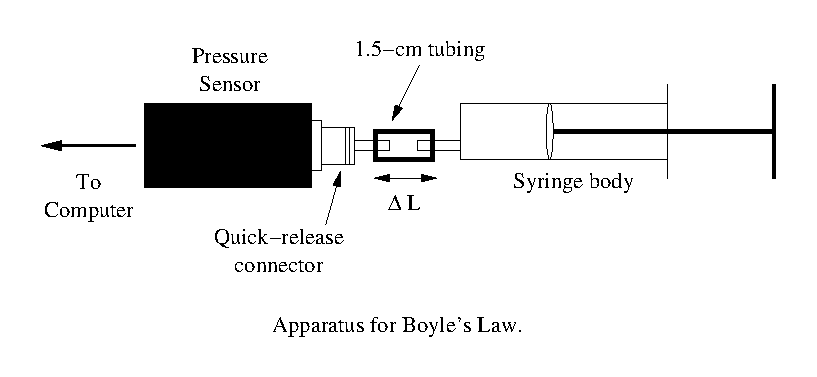
\includegraphics{boyles_law/boyleslawfig1.eps} \par}
\vspace{0.3cm}

\textbf{Introduction}

The behavior of a gas can be described in terms of the macroscopic quantities:
temperature (T), pressure (P), and volume (V). The relationship between these
quantities is given by the equation of state of the gas. A real gas behaves
approximately as an ideal gas if it is far from liquefaction. In that case,
the equation of state of an ideal gas can be used to describe a real gas. For
a given mass of a gas, if one of the quantities P, T, or V is changed, a change
in the other two quantities probably will result. However, if one of the quantities
is kept constant, the relationship between the other two can be studied. The
relationship between pressure and volume of an ideal gas is called Boyle's law.

The experimental apparatus is shown in the figure above. The gas is air contained
in a syringe that has marking on its side to measure the volume of the syringe.
A short tube connects the syringe with a pressure sensor that measures the pressure
in the tube and converts that measurement into a signal that can be read by
the DataStudio interface.

\textbf{Activity 1: Relationship Between P and V of a Gas}

(a) Check that there are no leaks in the apparatus by trying to compressing
the syringe from the 20.0 ml position to the 10.0 ml position. It should become
increasingly difficult to push the plunger as the volume decreases. If this
is not the case, check the couplings for fit. If no problem is obvious, then
consult your instructor. 
\vspace{20mm}

(b) The initial volume of air in the syringe should be set at 20.0 ml. If your
syringe is set to some other value, disconnect the quick release connector from
the sensor by gently rotating it in the counter-clockwise direction as you look
from the syringe toward the pressure sensor. Next, move the piston to the 20.0
ml position, and then re-connect the quick release connector to the pressure
sensor. 

(c) \textbf{Data Recording}. Open the Boyle's Law activity located in the 132
Workshop Folder under the {\bf Start} menu. Click on the window labeled \textit{Volume
and Pressure Table}. This is where your data will be displayed as you record
it. This table display will show the values of the gas volume in the syringe
which you will set by moving the piston to the appropriate marking on the syringe.
You will record the pressure at each of these settings with the pressure sensor.
To begin recording data, make sure the piston is at the 20-ml setting, and click
the Start button. The Start button will change to a Keep button and the table
display will show the value of the pressure next to the first volume value (20
ml) in the table. The reading in the pressure column should be colored red.
Click the Keep button to record this pressure (notice the reading in the Pressure
column beside the 20-ml entry changes from red to black). The next setting for
the volume (18 ml) will appear in the Volume column of the data table display.

NOTE: For the first pressure reading at 20 ml, the air in the syringe will be
in thermal equilibrium with the environment. This will not be the case immediately
after compressing the syringe for the next reading. Therefore, you must allow
a couple of seconds for the system to return to thermal equilibrium after you 
compress the syringe and before clicking on Keep to record pressure values. 

(d) Compress the syringe to the next value of the volume as listed in the data
display table (i.e., the window labeled \textit{Volume and Pressure Table})
and wait a couple of seconds for the system to reach thermal equilibrium. Once 
thermal equilibrium is reached, click Keep to record the pressure. The data 
table display will automatically change to show the next value of the volume 
at which the pressure will be measured. 

(e) Repeat step (d) for the remaining values of the volume listed in the table
display. In other words, continue taking pressure measurements at the prescribed
volume values in the data table display by moving the piston to the prescribed
value and clicking on Keep after thermal equilibrium is reached. After you record
the pressure for the last volume (8 ml), click the small, red box next to the
Keep button (this is the stop button) to end data recording.

(f) \textbf{Analysis.} What happened to the pressure when the volume was 
reduced from 20 ml to 8 ml? From looking at the data, do the pressure and 
volume seem to be directly or inversely proportional? Explain.
%Click on the GraphDisplay to examine the plots of Syringe
%Volume Reading vs. Pressure, and the Volume to Pressure ratio (as a function
%of measuring time). Print the GraphDisplay and attach it to this unit.
\vspace{25mm}

(g) Copy your data into a spreadsheet and plot pressure versus volume 
(including a title and axis labels with units). Next, fit your data with a 
trendline using a power function. Record the result here. What is the power of 
V? Print the graph and include it with this unit.
%What should you get for the power? Why?
\vspace{25mm}

(h) If pressure and volume are inversely proportional, then what can you say
about the product of pressure and volume? Explain.
\vspace{25mm}

\newpage

(i) The measurements you have made are V in milliliters (ml) and P in 
kilopascals (kPa). What are the corresponding units of PV? Show how you get 
this here (the result must be in energy units):
\vspace{40mm}

(j) Construct a table in the space below with the column headings: V (ml), P
(kPa), and PV. Include the units from above in the last column.
Enter the results for P and V in this new table and calculate
PV for each set of readings. Determine the mean value and the standard deviation
\( \sigma  \) for PV. Record the results in the form 
PV = Mean \( \pm \, \sigma  \). Be sure to include the proper units. 
What does this result tell you about the  product PV?

\vspace{12cm}

(k) Is there a trend in the values of PV as the volume decreases? If so, 
what do you suppose causes that trend?

%(j) Examine the plot on the next page with results from two different data 
%runs. How do you explain the difference between the curves for the different 
%tubing lengths (\( \triangle L \) in the diagram on the next page)?

%\vspace{40mm}

%\eject

%\vspace{0.3cm}
%{\par\centering 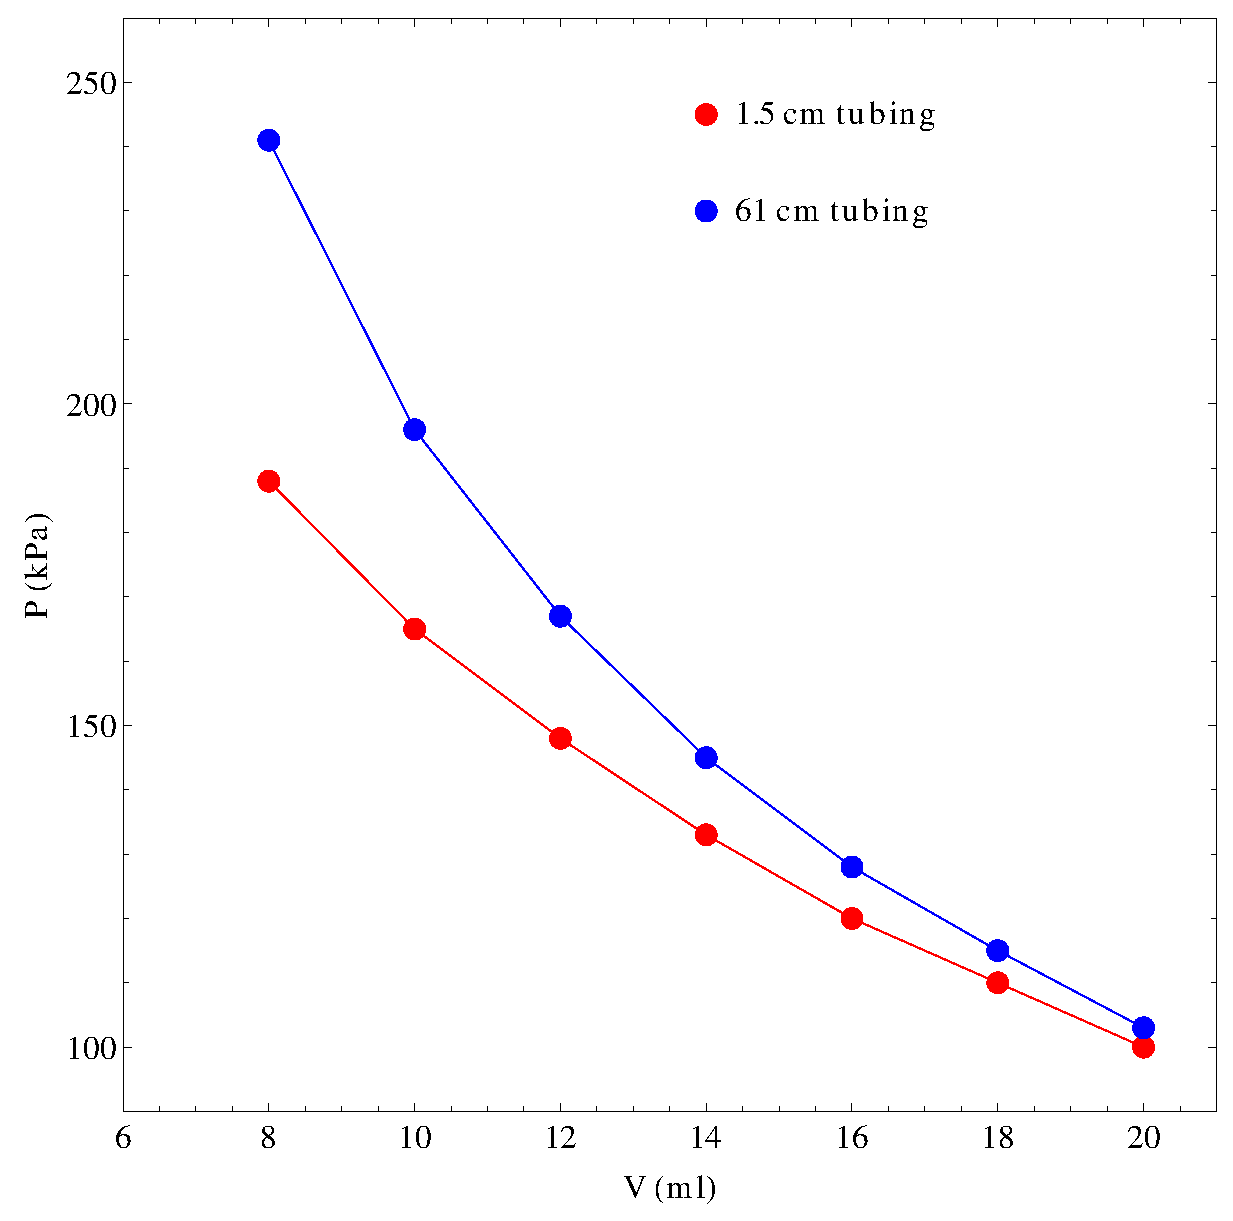
\includegraphics[width=6in]{boyles_law/PVfor132.eps} \par}
%\vspace{0.3cm}

%{\par\centering Results of measurement with Boyle's Law apparatus \par}

%{\par\centering different values of \( \triangle L \), the tubing length.\par}



\section{Charles' Law}

Name \rule{2.0in}{0.1pt}\hfill{}Section \rule{1.0in}{0.1pt}\hfill{}Date
\rule{1.0in}{0.1pt}+

\textbf{Objectives} 

To investigate the relationship between volume and temperature for
a constant mass of gas at constant pressure and determine the value
of absolute zero.

\textbf{Apparatus} 

\begin{itemize}
\item Charles law apparatus with stand.
\item Temperature sensor.
\item Air chamber, tubing, and ballast.
\item Containment vessel.
\end{itemize}
\vspace{0.3cm}

\begin{figure}[hbt]
\begin{center}
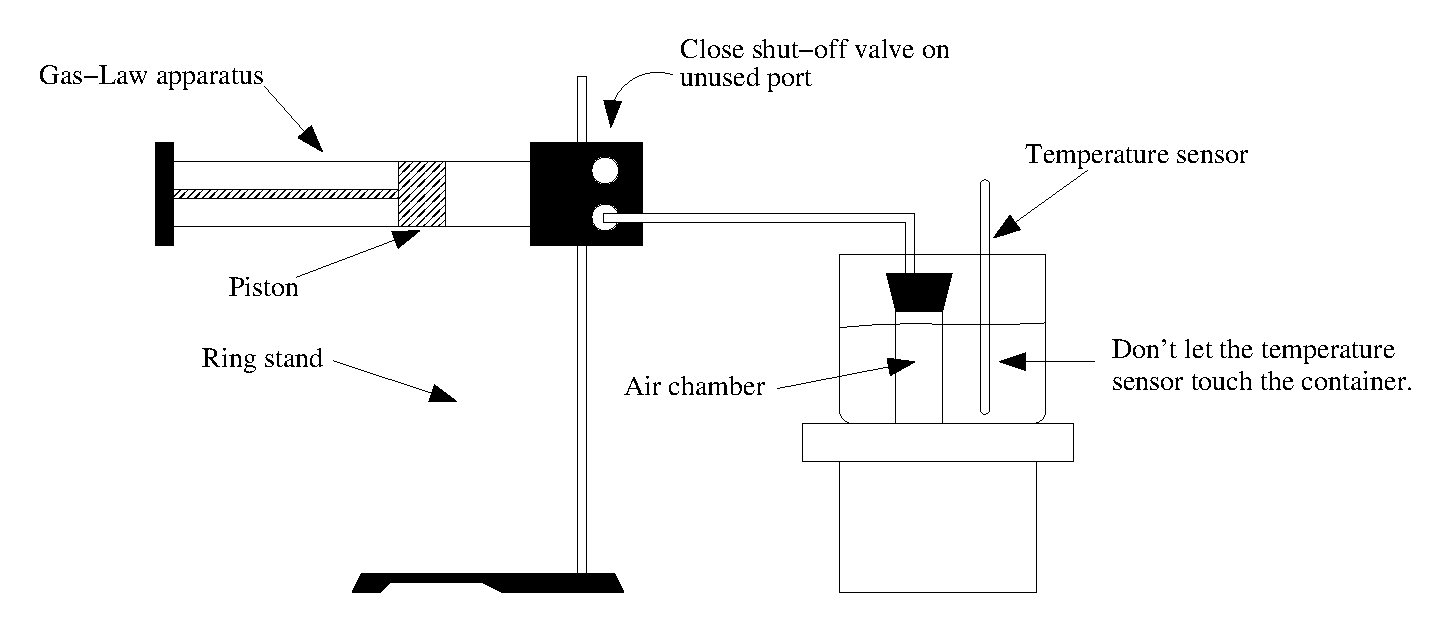
\includegraphics[width=6.0in]{charles_law_fig1.eps}
\caption{Charles' Law apparatus.}
\end{center}
\end{figure}

\textbf{Introduction}

The behavior of a gas can be described in terms of the macroscopic quantities:
temperature (T), pressure (P), and volume (V). The relationship between these
quantities is given by the equation of state of the gas. A real gas behaves
approximately as an ideal gas if it is far from liquefaction. In that case,
the equation of state of an ideal gas can be used to describe a real gas. For
a given mass of a gas, if one of the quantities P, T, or V is changed, a change
in the other two quantities probably will result. However, if one of the quantities
is kept constant, the relationship between the other two can be studied. The
relationship between temperature and volume of an ideal gas is called Charles' law.

The experimental apparatus is shown in the figure above and consists
of an air chamber containing dry air. The pressure on the air in the chamber is due to atmospheric
pressure applied through the movable piston.

\textbf{Activity 1: V-T Relationship for a Gas}

(a) Check that there are no leaks in the apparatus by trying to compressing
the piston from the 100 mm position to the 10 mm position. It should become
increasingly difficult to push the plunger as the volume decreases. If this
is not the case, check the couplings for fit. If no problem is obvious, then
consult your instructor. 

(b) Open the {\it Charles' Law} activity in the 132 Workshop Folder under the
{\bf Start} menu.
Click on the window labeled \textit{Charles' Law Table}. 
This is where your data will be displayed as you record
it. This table display will show the values of the gas temperature in the air chamber
and the entry number.
The data-taking procedure you will follow is described here first.
One member of your team will heat the air chamber in the flask on the hot plate 
and call out the position of the piston.
Another member will record the position settings by hand in the table below
and
click the {\bf Keep} button on the {\it DataStudio} interface to record the 
temperature for that entry.
To begin recording data, make sure the piston is at the low end of the scale, and click
the {\bf Start} button on the {\it DataStudio} interface. 
The {\bf Start} button will change to a {\bf Keep} button and the table
display will show the value of the temperature next to the first entry in the table. 
The reading in the temperature column should be colored red.
Click the {\bf Keep} button to record this temperature (notice the reading in the Temperature
column beside the entry number changes from red to black). The next entry number
 will appear in the Entry column of the data table display.

%NOTE: For the first temperature reading, the air in the chamber will be
%in thermal equilibrium with the environment. This will not be the case immediately
%after adding ice for the next reading. Therefore, you must allow
%3-5 seconds for the system to return to thermal equilibrium after you add ice
% and before clicking on {\bf Keep} to record temperature values. 

(c) Now, immerse the air chamber in a beaker of cold, tap water water and click
{\bf Start} on the {\it DataStudio} interface. You can monitor the temperature
on the temperature versus time plot to the right.
Make sure the set screw on the side of the piston is released.

(d) When the temperature is stable click {\bf Keep} and that point will be recorded in the
table. One team member should read off the piston position while the other 
writes it in the table at the same time.

(e) Now turn up the heat. The piston will move as the gas expands.
Read out the position of the piston every one or two millimeters. The other team member
will click {\bf Keep} (recording the temperature) and record the piston position
in the table.

(f) Repeat step (e) until the piston no longer moves or the water starts to boil.
 
(g) Calculate the volume of the apparatus for each piston position and plot
this volume versus temperature. The diameter of the Gas-Law apparatus is written on its
base.

\vspace{0.3cm}
{\centering \begin{tabular}{|c|c|c|c|}
\hline 
~~~Entry Number~~~&
~~~Piston Position (mm)~~~&
~~~Gas-Law Apparatus Volume (ml)~~~&
~~~Temperature ($^\circ  \rm C$)~~~\\
\hline
\hline 
&
&
&
\\
\hline 
&
&
&
\\
\hline 
&
&
&
\\
\hline 
&
&
&
\\
\hline 
&
&
&
\\
\hline 
&
&
&
\\
\hline 
&
&
&
\\
\hline 
&
&
&
\\
\hline 
&
&
&
\\
\hline
&
&
&
\\
\hline
&
&
&
\\
\hline
&
&
&
\\
\hline
&
&
&
\\
\hline
&
&
&
\\
\hline
\end{tabular}\par}
\vspace{0.3cm}

(h) How are the volume and temperature related?
Fit your data with the appropriate function and record the results here.
Print your plot and attach it to this unit.
\vspace{15mm}

(h) Repeat steps c-h to obtain a second {\it V-T} curve. Record your data in the table below
along with the fit to the V-T data.
\vspace{30mm}


\vspace{0.3cm}
{\centering \begin{tabular}{|c|c|c|c|}
\hline 
~~~Entry Number~~~&
~~~Piston Position (mm)~~~&
~~~Gas-Law Apparatus Volume (ml)~~~&
~~~Temperature ($^\circ  \rm C$)~~~\\
\hline
\hline 
&
&
&
\\
\hline 
&
&
&
\\
\hline 
&
&
&
\\
\hline 
&
&
&
\\
\hline 
&
&
&
\\
\hline 
&
&
&
\\
\hline 
&
&
&
\\
\hline 
&
&
&
\\
\hline 
&
&
&
\\
\hline
&
&
&
\\
\hline
&
&
&
\\
\hline
&
&
&
\\
\hline
&
&
&
\\
\hline
&
&
&
\\
\hline
\end{tabular}\par}
\vspace{2.0cm}

\textbf{Activity 2: Absolute Zero and the Kelvin Scale}

(a) The absolute zero of temperature can be defined as the temperature
at which the volume of an ideal gas is zero. Determine absolute
zero from the equations you obtained by fitting your V-T data.
\vspace{30mm}

(b) Determine the percent difference between your value of absolute
zero and the accepted value of -273\( ^{\circ } \)C. Are you happy or sad?
\vspace{30mm}

(c) Record the results from the other groups in class.
Obtain an average and standard deviation and record it here.
Are your results consistent with the class average? Explain.



\section{The \textit{P-T} Relationship of a Gas}

\makelabheader %(Space for student name, etc., defined in master.tex)

\bigskip
\textbf{Objectives} 

To investigate the relationship between pressure and temperature for
a constant mass of gas at constant volume and determine the value
of absolute zero.

\bigskip

\textbf{Apparatus} 

\begin{itemize}[nosep]
\item Pressure sensor
\item Temperature sensor
\item Air chamber and tubing
\item Hot plate
\item Glass beaker
\item Clamp and stand
\item Plastic beaker
\item Pasco 550 interface
\item \textit{Capstone} software (\filename{P-T.cap} experiment file)
\end{itemize}
\vspace{0.3cm}

\begin{figure}[hbt]
\begin{center}
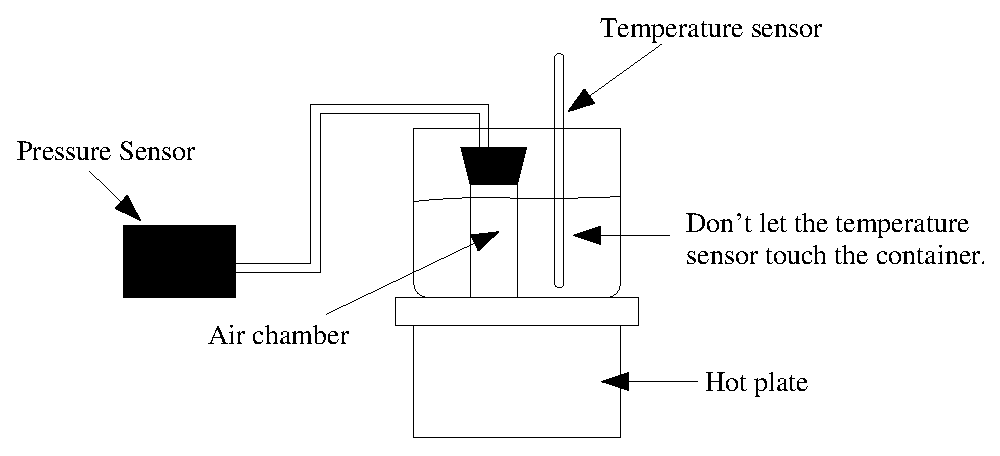
\includegraphics[width=6.0in]{P-T_relationship_of_gas/P-T_fig1b.eps}
\caption{P-T apparatus.}
\end{center}
\end{figure}

\textbf{Introduction}

The behavior of a gas can be described in terms of the macroscopic quantities:
temperature $T$, pressure $P$, and volume $V$. The relationship between these
quantities is given by the equation of state of the gas. A real gas behaves
approximately as an ideal gas if it is far from liquefaction. In that case,
the equation of state of an ideal gas can be used to describe a real gas. For
a given mass of a gas, if one of the quantities $P$, $T$, or $V$ is changed, a change
in the other two quantities probably will result. However, if one of the 
quantities is kept constant, the relationship between the other two can be 
studied. The relationship between temperature and pressure of an ideal gas is 
known as Gay-Lussac's law.

The experimental apparatus is shown in the figure above and consists
of an air chamber containing dry air. The volume of the gas is fixed. 
The temperature and pressure sensors are connected to the 550 Interface. 
Be sure the temperature sensor is connected to port A and the pressure sensor 
to port B. \textbf{Important:} Be sure the cables from the sensors are not touching the hot 
plate.

\bigskip

\pagebreak[2]
\textbf{Activity 1: $P$-$T$ Relationship for a Gas}

%(a) Fill the beaker 3/4 full with cold tap water and place it on the hot plate.  Immerse the air chamber in the water so that most of the volume of the air chamber is submerged.  The air chamber will have to be held in place with a clamp and stand or it will float to the top.  Set the temperature sensor in the water in such a way that it is not touching the side or bottom of the beaker.

(a) The equipment should be set when you arrive in lab. The air chamber is set 
inside the glass beaker on top of the hot plate. The temperature sensor is set 
so that it is not touching the side or bottom of the beaker. Use the plastic 
beaker to fill the glass beaker about 3/4 full of cold tap water.

(b) Open the file \filename{P-T.cap} in the \filename{\coursefolder} folder.
The graphs on the right display the temperature of the heat bath and the gas pressure as functions of time.  
The table on the left will record specific data points that you will choose.  
To begin recording data click
the \textit{Preview} button, which is where the \textit{Record} button usually would be. 
Once you hit \textit{Preview}, the current values of temperature and pressure will be coninuously graphed, and updated in the first row of the table.  When you hit the \textit{Keep Sample} button, the values at that time will be saved to the table, and you will continue to see current values displayed in the next row.


(c) Turn the hot plate on high.  As the temperature rises, click the \textit{Keep Sample} button when the temperature is 5-7\( ^{\circ } \) above its first value.  Continue recording the temperature and pressure at 5-7\( ^{\circ } \) intervals (by clicking the \textit{Keep Sample} button) until the water is close to boiling.  You can monitor the temperature on the temperature versus time plot to the right (on the monitor) or by watching the temperature in the \textit{Temperature and Pressure Table}.  After your last reading, click the \textit{Stop} button and turn off the hot plate.

(d) How are the pressure and temperature related?  Print your data table, enter the data in \textit{Excel} and plot pressure vs. temperature on a linear graph, showing the equation of the graph.  Print this graph and add it to this unit. Write the equation here as pressure $P$ as a function of temperature $T$, including UNITS on the constants.
\vspace{15mm}



\textbf{Activity 2: Absolute Zero and the Kelvin Scale}

(a) The absolute zero of temperature can be defined as the temperature
at which the pressure of an ideal gas is zero. Determine absolute
zero from the equation of your graph by setting $P = 0$ and solving for $T$.
\vspace{25mm}

(b) Record the results from the other groups in the class. 
Obtain an average and standard deviation and record it here.
Are your results consistent with the class average?  Explain.
\vspace{25mm}

(c) Does there appear to be a systematic error in the class results relative 
to the accepted value of $-273~^{\circ}$C?  If so, what do you suppose 
causes the error? Think about this and try to explain.




%--------------------------------------------
\appendix
\setcounter{section}{4} %set this counter to number MINUS ONE corresponding to desired appendix letter. (4 for `E', etc.)
%Put include statements for supplementary appendices below here.
\end{document}
